\section{Evaluation}
\label{sec:evaluation}

\subsection{Experiment setup}
We evaluate the flow scheduling on NCSU VCL \cite{VCL}.
In our evaluation, two types of nodes are includes:
1) 2 x 2.0GHz and 8GB memory, and 2) 4 x 2.4 GHz and 16GB memory.
Each of them is equipped with a 1-Gbps NIC.
We refer to the first group as Cluster 1 and the second groups as Cluster 2.
Both have Ubuntu 12.04 installed and Hadoop 2.0.3-alpha deployed.
One node in Cluster 2  is used for Resource Manger, and another one is for the name node of HDFS.
For computing facilities, two clusters are in different network segment, and Cluster 1 has six nodes and Cluster 2 has five nodes.
Regarding storage facilities, two data nodes of HDFS are in Cluster 1 and one is in Cluster 2.
Each has around 30GB disk space and we set the replication number of HDFS to two.

\subsection{Heterogeneous Cluster Setting}

We analyze the behavior of our flow scheduler and other existing Hadoop schedulers.
We compare Flow Scheduler with FIFO Scheduler, Fair Scheduler, and Capacity Scheduler.
Moreover, we create a Balancing Scheduler that distributes the flow demand to computing facilities evenly.
In this experiment, we setup a Hadoop system with Cluster 1 and Cluster 2.
Then we submit jobs (Wordcount, Terasort and Grep) to the Hadoop system every five seconds.
The wordcount and terasort job has an input size 1GB and we submit four times for each of them.
Since the grep job has longer running time, we submit only one job with input size 1GB.
As shown in Figure \ref{fig:het_elapsed}, FIFO Scheduler has the longest elapsed time and Flow Scheduler can complete all the jobs in a shorter time.
Figure \ref{fig:het_analysis} shows that Flow Scheduler has lower average execution time of tasks in most of cases.
Besides, Flow Scheduler demonstrates more smooth execution time of tasks, as shown in Figure \ref{fig:het_analysis_std}, because Flow Scheduler has lower values of the standard deviation of execution time.


\begin{figure}[ht]
    \centering
    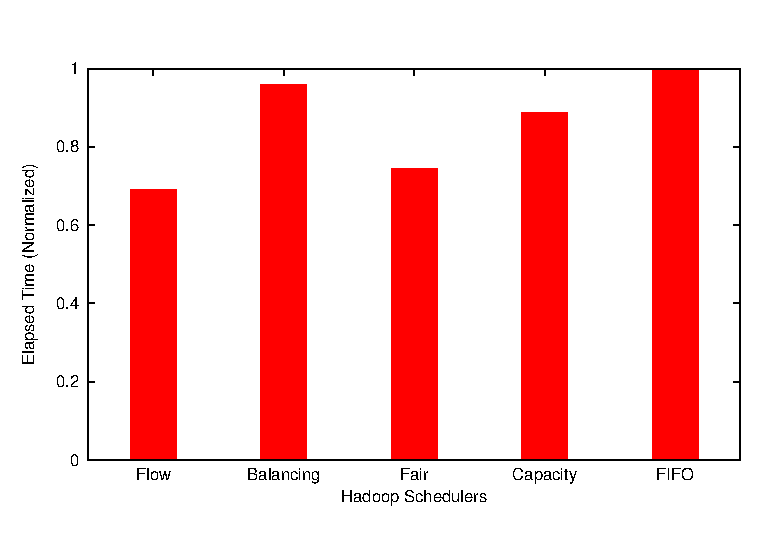
\includegraphics[width=0.8\textwidth]{figures/elapsed_time.eps}
    \caption{Elapsed time comparison.  The FIFO scheduler is the baseline.  Nine jobs with 1GB input are submitted every 5 second.}
    \label{fig:het_elapsed}
\end{figure}

\begin{figure}
    \centering
    \begin{subfigure}[b]{0.45\textwidth}
        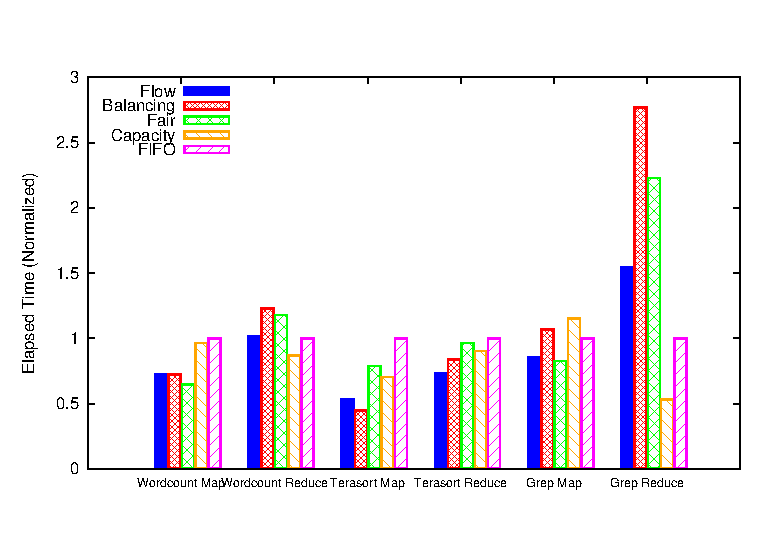
\includegraphics[width=\textwidth]{figures/avg_time.eps}
        \caption{Average of execution time}
        \label{fig:het_analysis_avg}
    \end{subfigure}
    %\par\bigskip
    ~ %add desired spacing between images, e. g. ~, \quad, \qquad, \hfill etc. 
      %(or a blank line to force the subfigure onto a new line)
    \begin{subfigure}[b]{0.45\textwidth}
        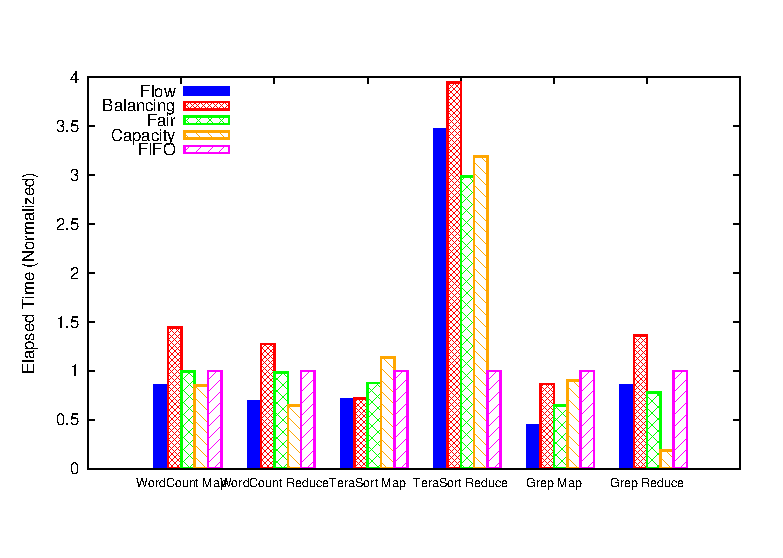
\includegraphics[width=\textwidth]{figures/std_time.eps}
        \caption{Standard deviation of execution time}
        \label{fig:het_analysis_std}
    \end{subfigure}
    \caption{The average execution time and the standard deviation of execution time.  Flow Scheduler shows more smooth execution time and this somehow suggests flow scheduling can eliminate stragglers that are caused by resource contention.}
    \label{fig:het_analysis}
\end{figure}


\subsection{Scheduling Overhead}
At each scheduling run, we filter out the computing facilities without available slots, and then calculate the penalty cost of each arc in the min-cost flow network.
This encoding is exported as an input to the solver to derive the optimal assignment.
The solver accounts most of scheduling overhead.
The graph size in our experiment is greater than $100$ at peak time ($|T|>100$ and $|C|=11$).
The maximum execution time is around $97ms$ and the minimum one is $2ms$, and the average solving time is $8.3ms$.
For a large-scale graph size, as indicated in \cite{IsardM2009_Quincy}, the solving time of the min-cost flow optimization problem can be acceptable.

\subsection{Discussion}

In the traditional Hadoop model, data locality plays an important role in system performance so that most existing schedulers focus on maximizing the number of local map tasks.
However, the decoupled Hadoop model does not have this property so that most existing schedulers does not fit in this model.
From our experiments, we observed that those schedulers might assign tasks directly to the first node with available slots, which happens on FIFO Scheduler more often.
FIFO Scheduler first considers node-level data locality and then rack-level data locality.
This scheduling method can cause problems because many tasks of a job would be assigned to a computing facility.
This would lead to resource competition especially when high flow demand of tasks are executed on the same node.
Figure \ref{fig:processing_flow_capability} shows a similar result when multiple higher flow demand tasks are running on a node.
The drop percentage appears to be the largest one for the  NoComputation line.

The proposed flow scheduling tries to avoid the task assignment that can affect the flow rate of processing.
Our cost model considers the quality of data supply ($R^{s}_{out}$ and $R^{c}_{out}$) and the qualify of processing flow rate on computing facilities.
We argue that maintaining the flow rate of processing can increase the system throughput, and Figure \ref{fig:processing_flow_capability} greatly support our argument.
More interestingly, our flow scheduling method can somehow eliminate stragglers \cite{DeanJ2004_MapReduce, ZahariaM2008_LATE}. 
Our result shows that Flow Scheduler derives more smooth execution time of map tasks.

Unlink the graph for the min-cost flow problem in Quincy \cite{IsardM2009_Quincy} and CAM \cite{LiM2012_CAM}, we do not construct a hierarchical graph to reflect the hierarchical data center networking.
The reason is that we can not convert our desired cost model into a hierarchical graph.
Suppose we take the top-of-rack switch into account, we introduce a new switch node $SW$.
We then construct an arc for each task assignment that produces data flow through $SW$.
We also construct another arc for computing facilities that connects to $SW$.
In such a scenario, we cannot decide the cost for the arc from $SW$ to $C_{m}$ because we lose the information of flow demand.
For this reason, Quincy has a cost, zero, for the arc from the rack to computing nodes.
In our cost model, we simply raise the cost of an arc that causes cross-rack communication.
To address this problem, we probably can look into convex network optimization that can support this scenario so as to delivering a more accurate cost model.
